\documentclass[aspectratio=169]{beamer}
\usepackage{color,amsmath}
\usepackage{subfigure}
\usepackage{booktabs}
\usepackage{framed}
\usepackage{comment}
\usepackage{hyperref}
\usepackage{ulem}

\usepackage{tikz}
\usetikzlibrary{arrows,shapes.arrows,positioning,shapes}
\newcommand\E{\text{E}}
\newcommand\blue[1]{{\color{blue}#1}}
\newcommand\bblue[1]{{\color{blue}\textbf{#1}}}
\newcommand\black[1]{{\color{black}#1}}
\newcommand\white[1]{{\color{white}#1}}
\usepackage{amsmath}

\usepackage{hyperref}
\hypersetup{
    colorlinks=true,
    linkcolor=blue,
    filecolor=magenta,      
    urlcolor=cyan,
}

%\usetheme{default}
%\beamertemplatenavigationsymbolsempty
%\usetikzlibrary{arrows,shapes.arrows,positioning,shapes}
%\usepackage{graphicx}
%\usepackage{hyperref}
%\usepackage{comment}
%\usepackage{ulem}
%
%\newcommand\red[1]{{\color{red}#1}}
%\newcommand\bred[1]{{\color{red}\textbf{#1}}}
%\newcommand\V{\text{V}}
%\renewcommand\P{\text{P}}
%

%%%%%%%%%%%%%%%%%%%%%%%%%%
\title[]{\textcolor{gray}{[Introduction to mass collaboration], [Human computation], [Open call], [Distributed data collection],} \newline [Fragile Families Challenge]}
\author[]{Matthew J. Salganik\\Department of Sociology\\Princeton University}
\date[]{%Summer Institutes in Computational Social Science\\2020
%\vfill
%\begin{flushleft}
%{\scriptsize
%The Summer Institutes in Computational Social Science is supported by grants from the Russell Sage Foundation and the Alfred P. Sloan Foundation.}
%\end{flushleft}
\begin{flushright}

\includegraphics[width=0.1\textwidth]{figures/cc-by.png}
\end{flushright}
}
\begin{document}
%%%%%%%%%%%%%%%%%%%%%%%%%%
\frame{\titlepage}
%%%%%%%%%%%%%%%%%%%%%%%%%%
\begin{frame}

\begin{columns}
\begin{column}{.40\textwidth}
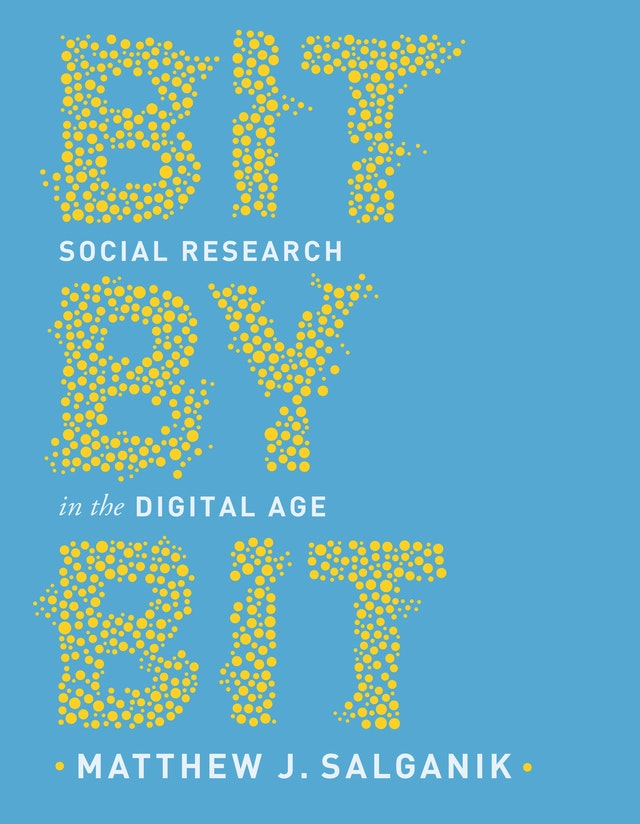
\includegraphics[width=\textwidth]{figures/salganik_bit_2018_cover}
\end{column}%

\hfill%

\begin{column}{.60\textwidth}
1) Introduction \\
2) Observing behavior \\
3) Asking questions \\
4) Running experiments \\
\textcolor{blue}{5) Mass collaboration} \\
6) Ethics \\
7) The future \\
\end{column}%
\end{columns}

\end{frame}
%%%%%%%%%%%%%%%%%%%%%%%%%
\begin{frame}

\begin{center}
\only<1>{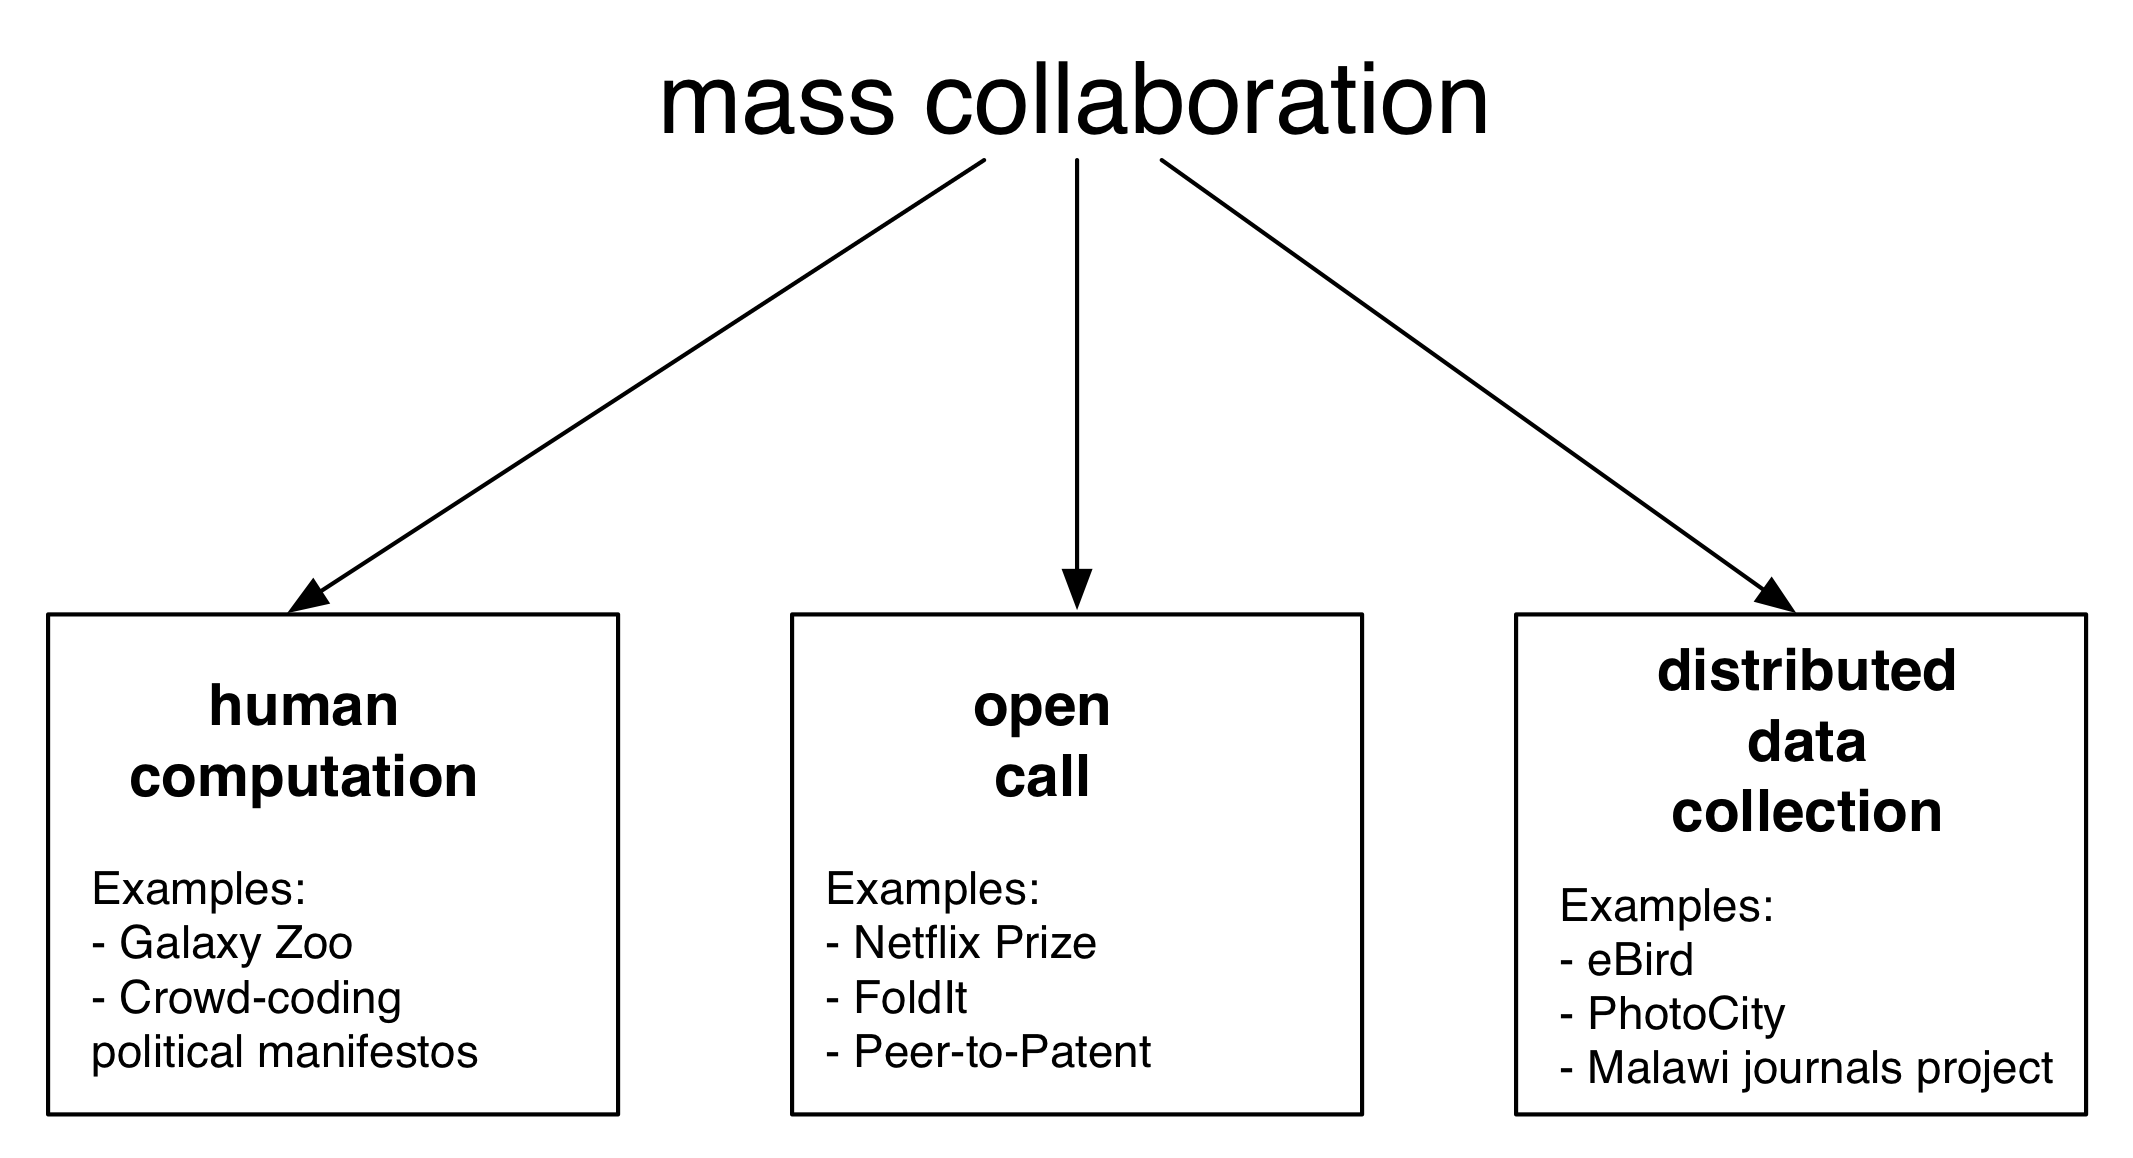
\includegraphics[width=0.9\textwidth]{figures/mass_collaboration_schematic}}
\only<2>{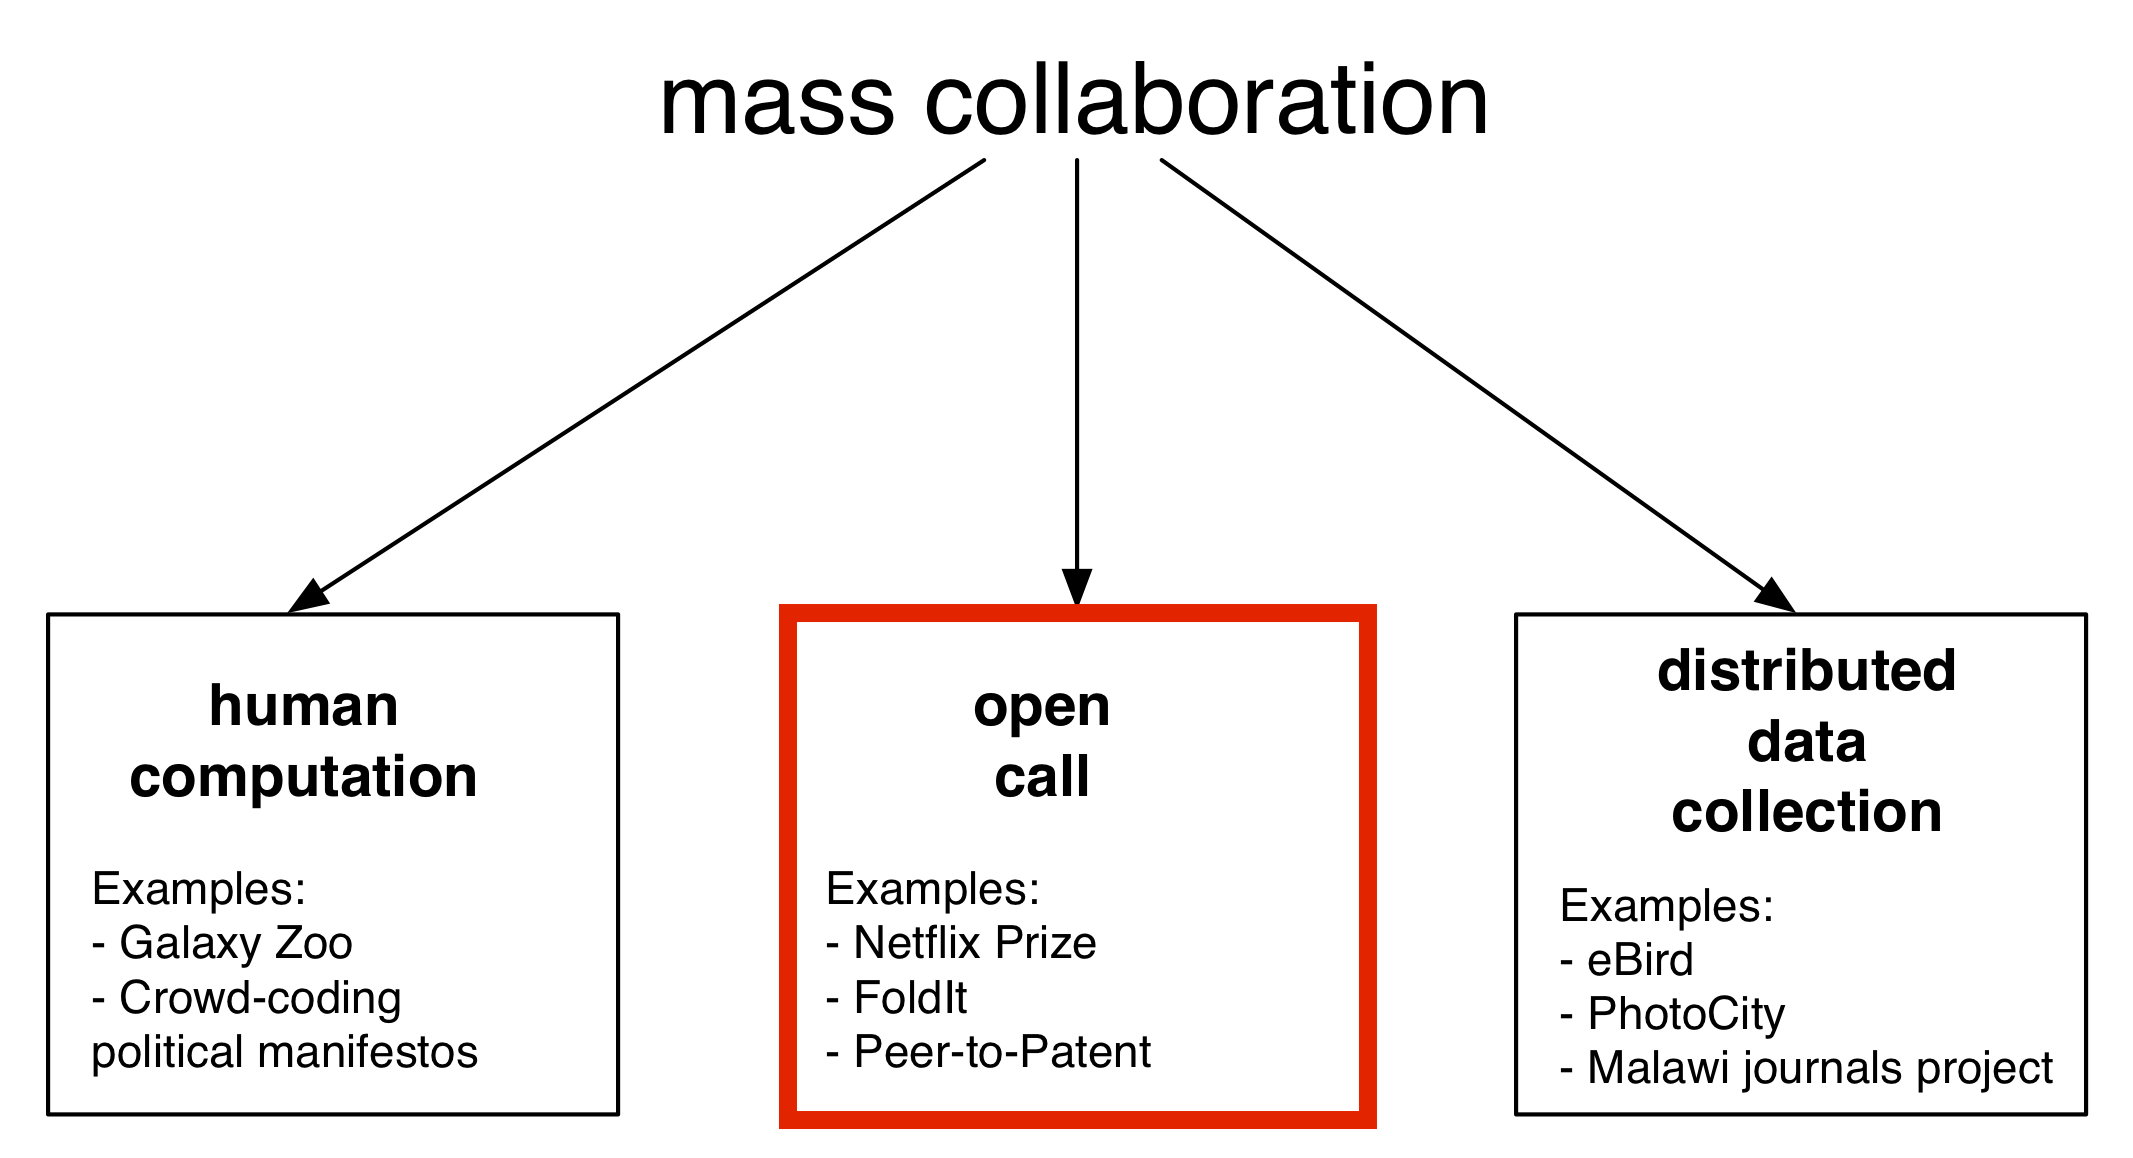
\includegraphics[width=0.9\textwidth]{figures/mass_collaboration_schematic_open_call}}
\end{center}

\vfill
Fig 5.4 (\href{https://www.bitbybitbook.com/}{Salganik 2018})
\end{frame}

%%%%%%%%%%%%%%%%%%%%%%%%%%
\title{Measuring the Predictability of Life Outcomes with a Scientific Mass Collaboration}

\author{{\small Matthew Salganik, Ian Lundberg, Alex Kindel, Sara McLanahan,\\and the participants in the Fragile Families Challenge}}

\institute[]{}
\date{\vfill
\begin{flushleft}{\tiny Funding for FFCWS provided by NICHD (R01HD36916, R01HD39135, R01HD40421) and a consortium of private foundations, including the Robert Wood Johnson Foundation. Funding for FFC provided by the Russell Sage Foundation, NSF, \& the Overdeck Fund. FFC Board of Advisors: Jeanne Brooks-Gunn, Kathryn Edin, Barbara Engelhardt, Irwin Garfinkel, Moritz Hardt, Dean Knox, Nicholas Lemann, Karen Levy, Sara McLanahan, Arvind Narayanan, Timothy Nelson, Matthew Salganik, Brandon Stewart \& Duncan Watts.}
\end{flushleft}
}

%%%%%%%%%%%%%%%%%%%%%%%%%%%%%%
\begin{frame}
  \titlepage
\end{frame}
%%%%%%%%%%%%%%%%%%%%%%%%%%%
\begin{frame}

\begin{center}
\includegraphics[width=0.6\textwidth]{figures/wikipedia_logo}
\end{center}

\end{frame}
%%%%%%%%%%%%%%%%%%%%%%%%%%%
\begin{frame}

\begin{center}
\includegraphics[width=0.9\textwidth]{figures/lander_initial_2001_title}
\end{center}

\vfill
{\tiny \url{http://dx.doi.org/10.1038/35057062}}

\end{frame}
%%%%%%%%%%%%%%%%%%%%%%%%%%
\begin{frame}

\begin{center}
\includegraphics[height=0.9\textheight]{figures/lander_initial_2001_authors}
\end{center}

\end{frame}
%%%%%%%%%%%%%%%%%%%%%%%%%%
\begin{frame}

\begin{center}
\includegraphics[width=\textwidth]{figures/aad_combined_2015_title}
\end{center}

\vfill
{\tiny \url{https://doi.org/10.1103/PhysRevLett.114.191803}}

\end{frame}
%%%%%%%%%%%%%%%%%%%%%%%%%%
\begin{frame}

\begin{center}
\only<1>{\includegraphics[height=\textheight]{figures/aad_combined_2015_authors_01}}%
\only<2>{\includegraphics[height=\textheight]{figures/aad_combined_2015_authors_02}}%
\only<3>{\includegraphics[height=\textheight]{figures/aad_combined_2015_authors_03}}%
\only<4>{\includegraphics[height=\textheight]{figures/aad_combined_2015_authors_04}}%
\only<5>{\includegraphics[height=\textheight]{figures/aad_combined_2015_authors_05}}%
\only<6>{\includegraphics[height=\textheight]{figures/aad_combined_2015_authors_06}}%
\only<7>{\includegraphics[height=\textheight]{figures/aad_combined_2015_authors_07}}%
\only<8>{\includegraphics[height=\textheight]{figures/aad_combined_2015_authors_08}}%
\only<9>{\includegraphics[height=\textheight]{figures/aad_combined_2015_authors_09}}%
\only<10>{\includegraphics[height=\textheight]{figures/aad_combined_2015_authors_10}}%
\only<11>{\includegraphics[height=\textheight]{figures/aad_combined_2015_authors_11}}%
\only<12>{\includegraphics[height=\textheight]{figures/aad_combined_2015_authors_12}}%
\only<13>{\includegraphics<13>[height=\textheight]{figures/aad_combined_2015_authors_13}}%
\only<14>{\includegraphics<14>[height=\textheight]{figures/aad_combined_2015_authors_14}}%
\only<15>{\includegraphics<15>[height=\textheight]{figures/aad_combined_2015_authors_15}}%
\only<16>{\includegraphics<16>[height=\textheight]{figures/aad_combined_2015_authors_16}}%
\only<17>{\includegraphics<17>[height=\textheight]{figures/aad_combined_2015_authors_17}}%
\only<18>{\includegraphics<18>[height=\textheight]{figures/aad_combined_2015_authors_18}}%
\only<19>{\includegraphics<19>[height=\textheight]{figures/aad_combined_2015_authors_19}}%
\only<20>{\includegraphics<20>[height=\textheight]{figures/aad_combined_2015_authors_20}}%
\only<21>{\includegraphics<21>[height=\textheight]{figures/aad_combined_2015_authors_21}}%
\only<22>{\includegraphics<22>[height=\textheight]{figures/aad_combined_2015_authors_22}}%
\only<23>{\includegraphics<23>[height=\textheight]{figures/aad_combined_2015_authors_23}}%
\only<24>{\includegraphics<24>[height=\textheight]{figures/aad_combined_2015_authors_24}}%
\only<25>{\includegraphics<25>[height=\textheight]{figures/aad_combined_2015_authors_25}}
\end{center}

\end{frame}
%%%%%%%%%%%%%%%%%%%%%%%%%
\begin{frame}

\begin{center}
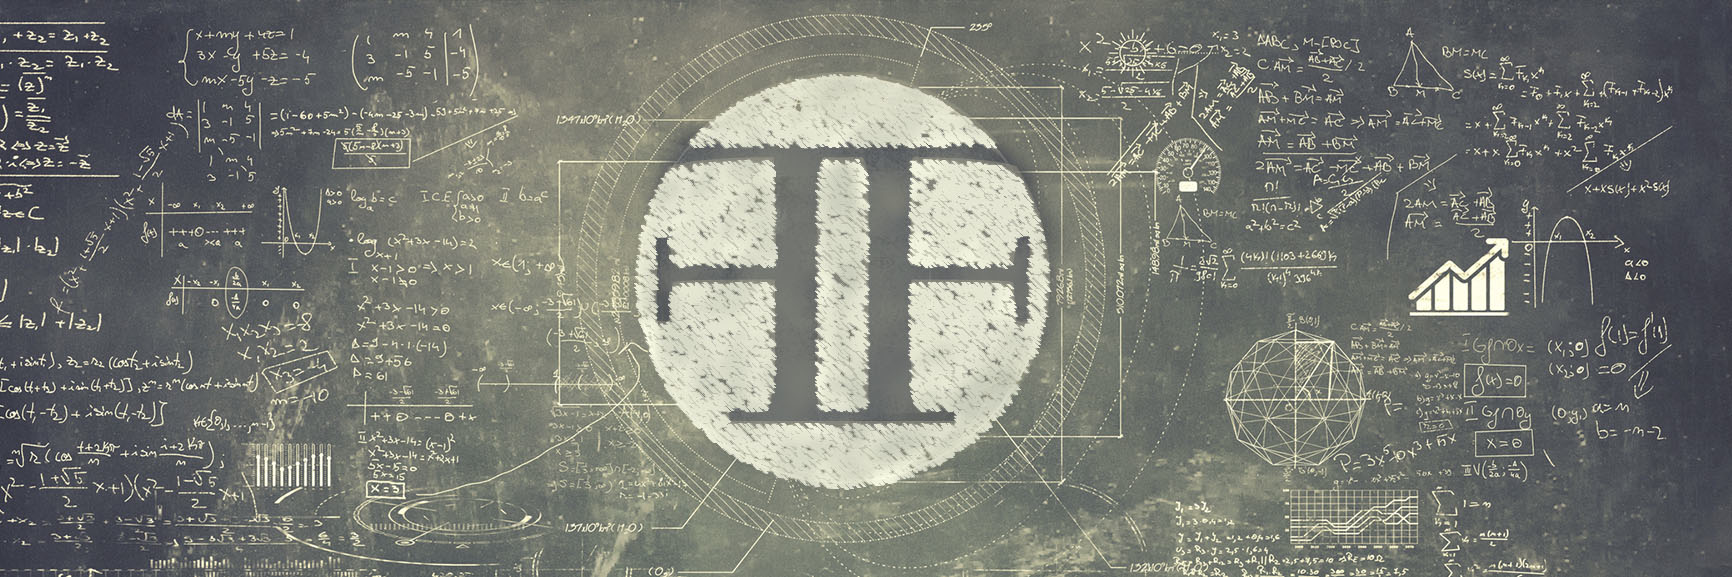
\includegraphics[width=\textwidth]{figures/ffc_masthead}
\Large{Fragile Families Challenge}
\end{center}

\end{frame}
%%%%%%%%%%%%%%%%%%%%%%%%%%%
\begin{frame}
\centering
\begin{tikzpicture}[x = .5\textwidth, y = .5\textheight]
\node at (-1,-1) {};
\node at (1,1) {};
\node[font = \Large] at (0,.8) {An overly simple view of stratification research.};
\onslide<1-1>{
	\node[font = \Huge] at (0,.5) {$Y = \white{\underbrace{\black{\E\left(Y\mid \vec{X}\right)}}} + \epsilon$};
}
\onslide<8->{
	\node[font = \Huge] at (0,.5) {$Y = \underbrace{\E\left(Y\mid \vec{X}\right)} + \hspace{5pt}\epsilon$};
}
\onslide<2-3>{
	\node[font = \Huge] at (0,.5) {$\blue{Y} = \white{\underbrace{\black{\E\left(Y\mid \vec{X}\right)}}} + \epsilon$};
}
\onslide<4-5,7>{
	\node[font = \Huge] at (0,.5) {$Y = \blue{\underbrace{\E\left(Y\mid \vec{X}\right)}} + \epsilon$};
}
\onslide<6>{
	\node[font = \Huge] at (0,.5) {$Y = \blue{\underbrace{\beta_1X_1 + \beta_2X_2}} + \epsilon$};
}
\onslide<8-9>{
	\node[font = \Huge] at (0,.5) {$Y = \underbrace{\E\left(Y\mid \vec{X}\right)} +\blue{\hspace{5pt}\epsilon}$};
}
\onslide<2-3>{
	\node[font = \Large,blue,anchor=west] (attainment) at (-1,.2) {\bblue{Attainment}};
	\draw[->, line width = 1.5pt, blue] (-.6,0.4) -- (attainment);
}
\onslide<3-3>{
	\node[font = \Large,blue,anchor = west,align=left] (achievement) at (-1,0) {-- Academic\\\hspace{13pt}achievement};
	\node[font = \Large,blue,anchor = west] (occupation) at (-1,-.22) {-- Occupation};
	\node[font = \Large,blue,anchor = west] (income) at (-1,-.37) {-- Income};
}
\onslide<4-9>{
	\node[font = \Large,black,anchor = west,align=left] (achievement) at (-1,0) {-- Academic\\\hspace{13pt}achievement};
	\node[font = \Large,black,anchor = west] (occupation) at (-1,-.22) {-- Occupation};
	\node[font = \Large,black,anchor = west] (income) at (-1,-.37) {-- Income};
}
\onslide<4->{
	\node[font = \Large,anchor=west] (attainment) at (-1,.2) {\textbf{Attainment}};
	\draw[->, line width = 1.5pt] (-.6,0.4) -- (attainment);
}
\onslide<4-7>{
	\node[font = \Large,blue,anchor=north,align=center] (predictable) at (0.04,.15) {\bblue{Predictable}\\\bblue{component}};
	\draw[->, line width = 1.5pt, blue] (0.04, 0.25) -- (predictable);
}
\onslide<8->{
	\node[font = \Large,anchor=north,align=center] (predictable) at (0.04,.15) {\textbf{Predictable}\\\textbf{component}};
	\draw[->, line width = 1.5pt] (0.04, 0.25) -- (predictable);
}
\onslide<8-9>{
	\node[font = \Large,align=center,blue] (unpredictable) at (.7,.1) {\bblue{Unpredictable}\\\bblue{component}};
	\draw[->, line width = 1.5pt, blue] (.63,0.4) -- (unpredictable);
}
\onslide<10->{
	\node[font = \Large,align=center] (unpredictable) at (.7,.1) {\textbf{Unpredictable}\\\textbf{component}};
	\draw[->, line width = 1.5pt] (0.63,0.4) -- (unpredictable);
}
\onslide<10->{
	\node[font = \Large,anchor = west] at (-1.05,-.25) {Theories focus on the predictable component, but};
}
\onslide<10->{
	\node[font = \Large,anchor = west] at (-1.05,-.4) {empirically the unpredictable component dominates};
}
\end{tikzpicture}
\end{frame}
%%%%%%%%%%%%%%%%%%%%%%%%%%%%%%%
\begin{frame}

\begin{center}
\LARGE{
$ \hat{y} \quad \& \quad \hat{\beta}$
}
\end{center}

\vfill
\small{Mullainathan and Spiess (2017): \url{http://dx.doi.org/10.1257/jep.31.2.87}}
\end{frame}
%%%%%%%%%%%%%%%%%%%%%%%%%%
\begin{frame}

We should care about the predictability of social outcomes\pause
\begin{itemize}
\item Scientific reasons \pause
\begin{itemize}
\item Basic social fact
\item Discovery \pause
\end{itemize}
\item Policy reasons
\begin{center}
\includegraphics[width=0.8\textwidth]{figures/hurley_can_2018_title} 
\end{center}
\end{itemize}

\end{frame}
%%%%%%%%%%%%%%%%%%%%%%%%%
\begin{frame}

\begin{center}
\includegraphics[width=\textwidth]{figures/ff_logo}
\end{center}

\begin{itemize}
\item Birth cohort panel study
\item $\approx$ 5,000 children born in 20 U.S. cities with an over-sample of non-marital births
\item Followed from birth through age 15
\item Already used in hundreds of papers and dozens of dissertations
\end{itemize}

\end{frame}
%%%%%%%%%%%%%%%%%%%%%%%%%%%
\begin{frame}

\begin{center}
\only<1>{\includegraphics[width=0.8\textwidth]{figures/ff_design_public_b9}}
\only<2>{\includegraphics[width=0.8\textwidth]{figures/ff_design_public2}}
\end{center}

\end{frame}
%%%%%%%%%%%%%%%%%%%%%%%%%
\begin{frame}

\begin{center}
\includegraphics[width=\textwidth]{figures/ff_design_matrix_ml}
\end{center}

\end{frame}
%%%%%%%%%%%%%%%%%%%%%%%%%
\begin{frame}

\begin{center}
\includegraphics[width=\textwidth]{figures/ffc_design_matrix_ml}
\end{center}

\end{frame}
%%%%%%%%%%%%%%%%%%%%%%%%%
\begin{frame}

Outcomes
\begin{itemize}
\item Child: GPA (continuous), Grit (continuous)
\item Household:  Eviction (binary), Material hardship (continuous)
\item Primary care giver: Job training (binary), Job loss (binary)
\end{itemize}

\end{frame}
%%%%%%%%%%%%%%%%%%%%%%%%%
\begin{frame}

457 researchers applied to participate. Many worked in interdisciplinary teams. Goal: Make a prediction that minimizes mean square error on the hold-out set
\begin{equation*}
MSE_{\text{holdout}} = \frac{\sum_{i \in \text{holdout}} (\hat{y}_i - y_i)^2}{n_{holdout}}
\end{equation*}

\vfill
More on privacy and ethics audit: \href{https://doi.org/10.1177/2378023118813023}{Lundberg et al.\ (2019)}
\end{frame}
%%%%%%%%%%%%%%%%%%%%%%%%%
\begin{frame}

Using a large, high-quality social science dataset collected since birth and modern machine learning methods, how accurately can we predict outcomes from children, parents, and families?

\begin{equation*}
R^2_{holdout} = 1 - \frac{\sum_{i \in \text{holdout}} (\hat{y}_i - y_i)^2}{\sum_{i \in \text{holdout}} (\bar{y}_{train} - y_i)^2}
\end{equation*}

\pause 
\vfill

Before I show the results, let's vote . . . .

\end{frame}
%%%%%%%%%%%%%%%%%%%%%%%%%
\begin{frame}

\begin{center}
\only<1>{\includegraphics[width=0.95\textwidth]{figures/RSquared_all_ASA.pdf}}
\only<2>{\includegraphics[width=0.95\textwidth]{figures/RSquared_all_ASA_01.pdf}}
\end{center}

\end{frame}
%%%%%%%%%%%%%%%%%%%%%%
\begin{frame}

\begin{center}
\Large{Is this even better than a benchmark model?}
\end{center}

\end{frame}
%%%%%%%%%%%%%%%%%%%
\begin{frame}

\begin{center}
\only<1>{\includegraphics[width=0.95\textwidth]{figures/RSquared_all_ASA_01.pdf}} %
\only<2>{\includegraphics[width=0.95\textwidth]{figures/RSquared_all_ASA_01_benchmark.pdf}} %
\end{center}

\vfill 

\onslide<2>{Green line: 4 variable linear regression model}

\end{frame}
%%%%%%%%%%%%%%%%%%%%%%%%%%%
\begin{frame}

\begin{center}
\only<1>{\includegraphics[width=0.7\textwidth]{figures/materialhardship_scatter_best_benchmark}} %
\only<2>{\includegraphics[width=0.9\textwidth]{figures/allcontinuous_scatter_best_benchmark}} %
\end{center}

\end{frame}
%%%%%%%%%%%%%%%%%%%%%%%%%%%
\begin{frame}

\begin{center}
\only<1>{\includegraphics[width=0.7\textwidth]{figures/eviction_density_best_benchmark}} %
\only<2>{\includegraphics[width=0.9\textwidth]{figures/allbinary_density_best_benchmark}} %
\end{center}

\end{frame}
%%%%%%%%%%%%%%%%%%%%%%%%%%%
\begin{frame}

\begin{center}
\Large{What can we learn looking at all the predictions?}
\end{center}

\end{frame}
%%%%%%%%%%%%%%%%%%%
\begin{frame}

\begin{center}
\includegraphics[height=0.90\textheight]{figures/materialHardship_ysort_mse_unit_outcome_xsort_mse_account_outcome.pdf}
\end{center}

\end{frame}
%%%%%%%%%%%%%%%%%%%%%%%%%%
\begin{frame}

\begin{center}
\includegraphics[width=0.20\textwidth]{figures/materialHardship_ysort_mse_unit_outcome_xsort_mse_account_outcome.pdf}
\includegraphics[width=0.20\textwidth]{figures/gpa_ysort_mse_unit_outcome_xsort_mse_account_outcome.pdf}
\includegraphics[width=0.20\textwidth]{figures/grit_ysort_mse_unit_outcome_xsort_mse_account_outcome.pdf} \\
\includegraphics[width=0.20\textwidth]{figures/eviction_ysort_mse_unit_outcome_xsort_mse_account_outcome.pdf}
\includegraphics[width=0.20\textwidth]{figures/jobtraining_ysort_mse_unit_outcome_xsort_mse_account_outcome.pdf}
\includegraphics[width=0.20\textwidth]{figures/layoff_ysort_mse_unit_outcome_xsort_mse_account_outcome.pdf}
\end{center}

\end{frame}
%%%%%%%%%%%%%%%%%%%%%%%%%%
\begin{frame}

\begin{center}
\Large{What do these results mean for policy makers?}
\end{center}

\end{frame}
%%%%%%%%%%%%%%%%%%%%%%%%%%%%
\begin{frame}

\begin{itemize}
\item Machine learning is not magic\pause
\item Transparent evaluation of any algorithm is needed \pause
\item Complex models may not outperform simple models
\end{itemize}

\end{frame}
%%%%%%%%%%%%%%%%%%%%%%%%%%%%
\begin{frame}

\begin{center}
\Large{What do these results mean for researchers?}
\end{center}

\end{frame}
%%%%%%%%%%%%%%%%%%%%%%%%%%%%
\begin{frame}

Researchers must reconcile an ``understanding/prediction'' paradox \pause
\begin{itemize}
\item We don't understand much \pause
\item Prediction is not a good measure of understanding \pause
\item Our current understanding is correct but incomplete
\end{itemize}

\end{frame}
%%%%%%%%%%%%%%%%%%%%%%%%%%%%
\begin{frame}

\begin{center}
{\Large How can we expand our understanding?}\\ 
\vspace{0.5in}
\pause
{\Large In-depth, semi-structured interviews}
\end{center}

\vfill
Dark matter interview team: Rachel M. Brown-Weinstock, Bobbi Brashear, Kristin Catena, Susan Clampet-Lundquist, Sophie Damas, Katie Donnalley, Kaitlin Edin-Nelson, Kathryn Edin, Alexus Fraser, Sarah Gold, Ashley Hyman, Daniel Kim, Ian Lundberg, Abigail MacLean, Collin ``Ren'' MacLean, Stefanie Mavronis, Timothy Nelson, Matthew Salganik, Naomi Shifrin, and Vicki Yang.
\end{frame}
%%%%%%%%%%%%%%%%%%%%%%%%%%%
\begin{frame}

\begin{center}
\includegraphics[width=\textwidth]{figures/kaizen_cycle}
\end{center}

\end{frame}
%%%%%%%%%%%%%%%%%%%%%%%%%%%
\begin{frame}

\begin{center}
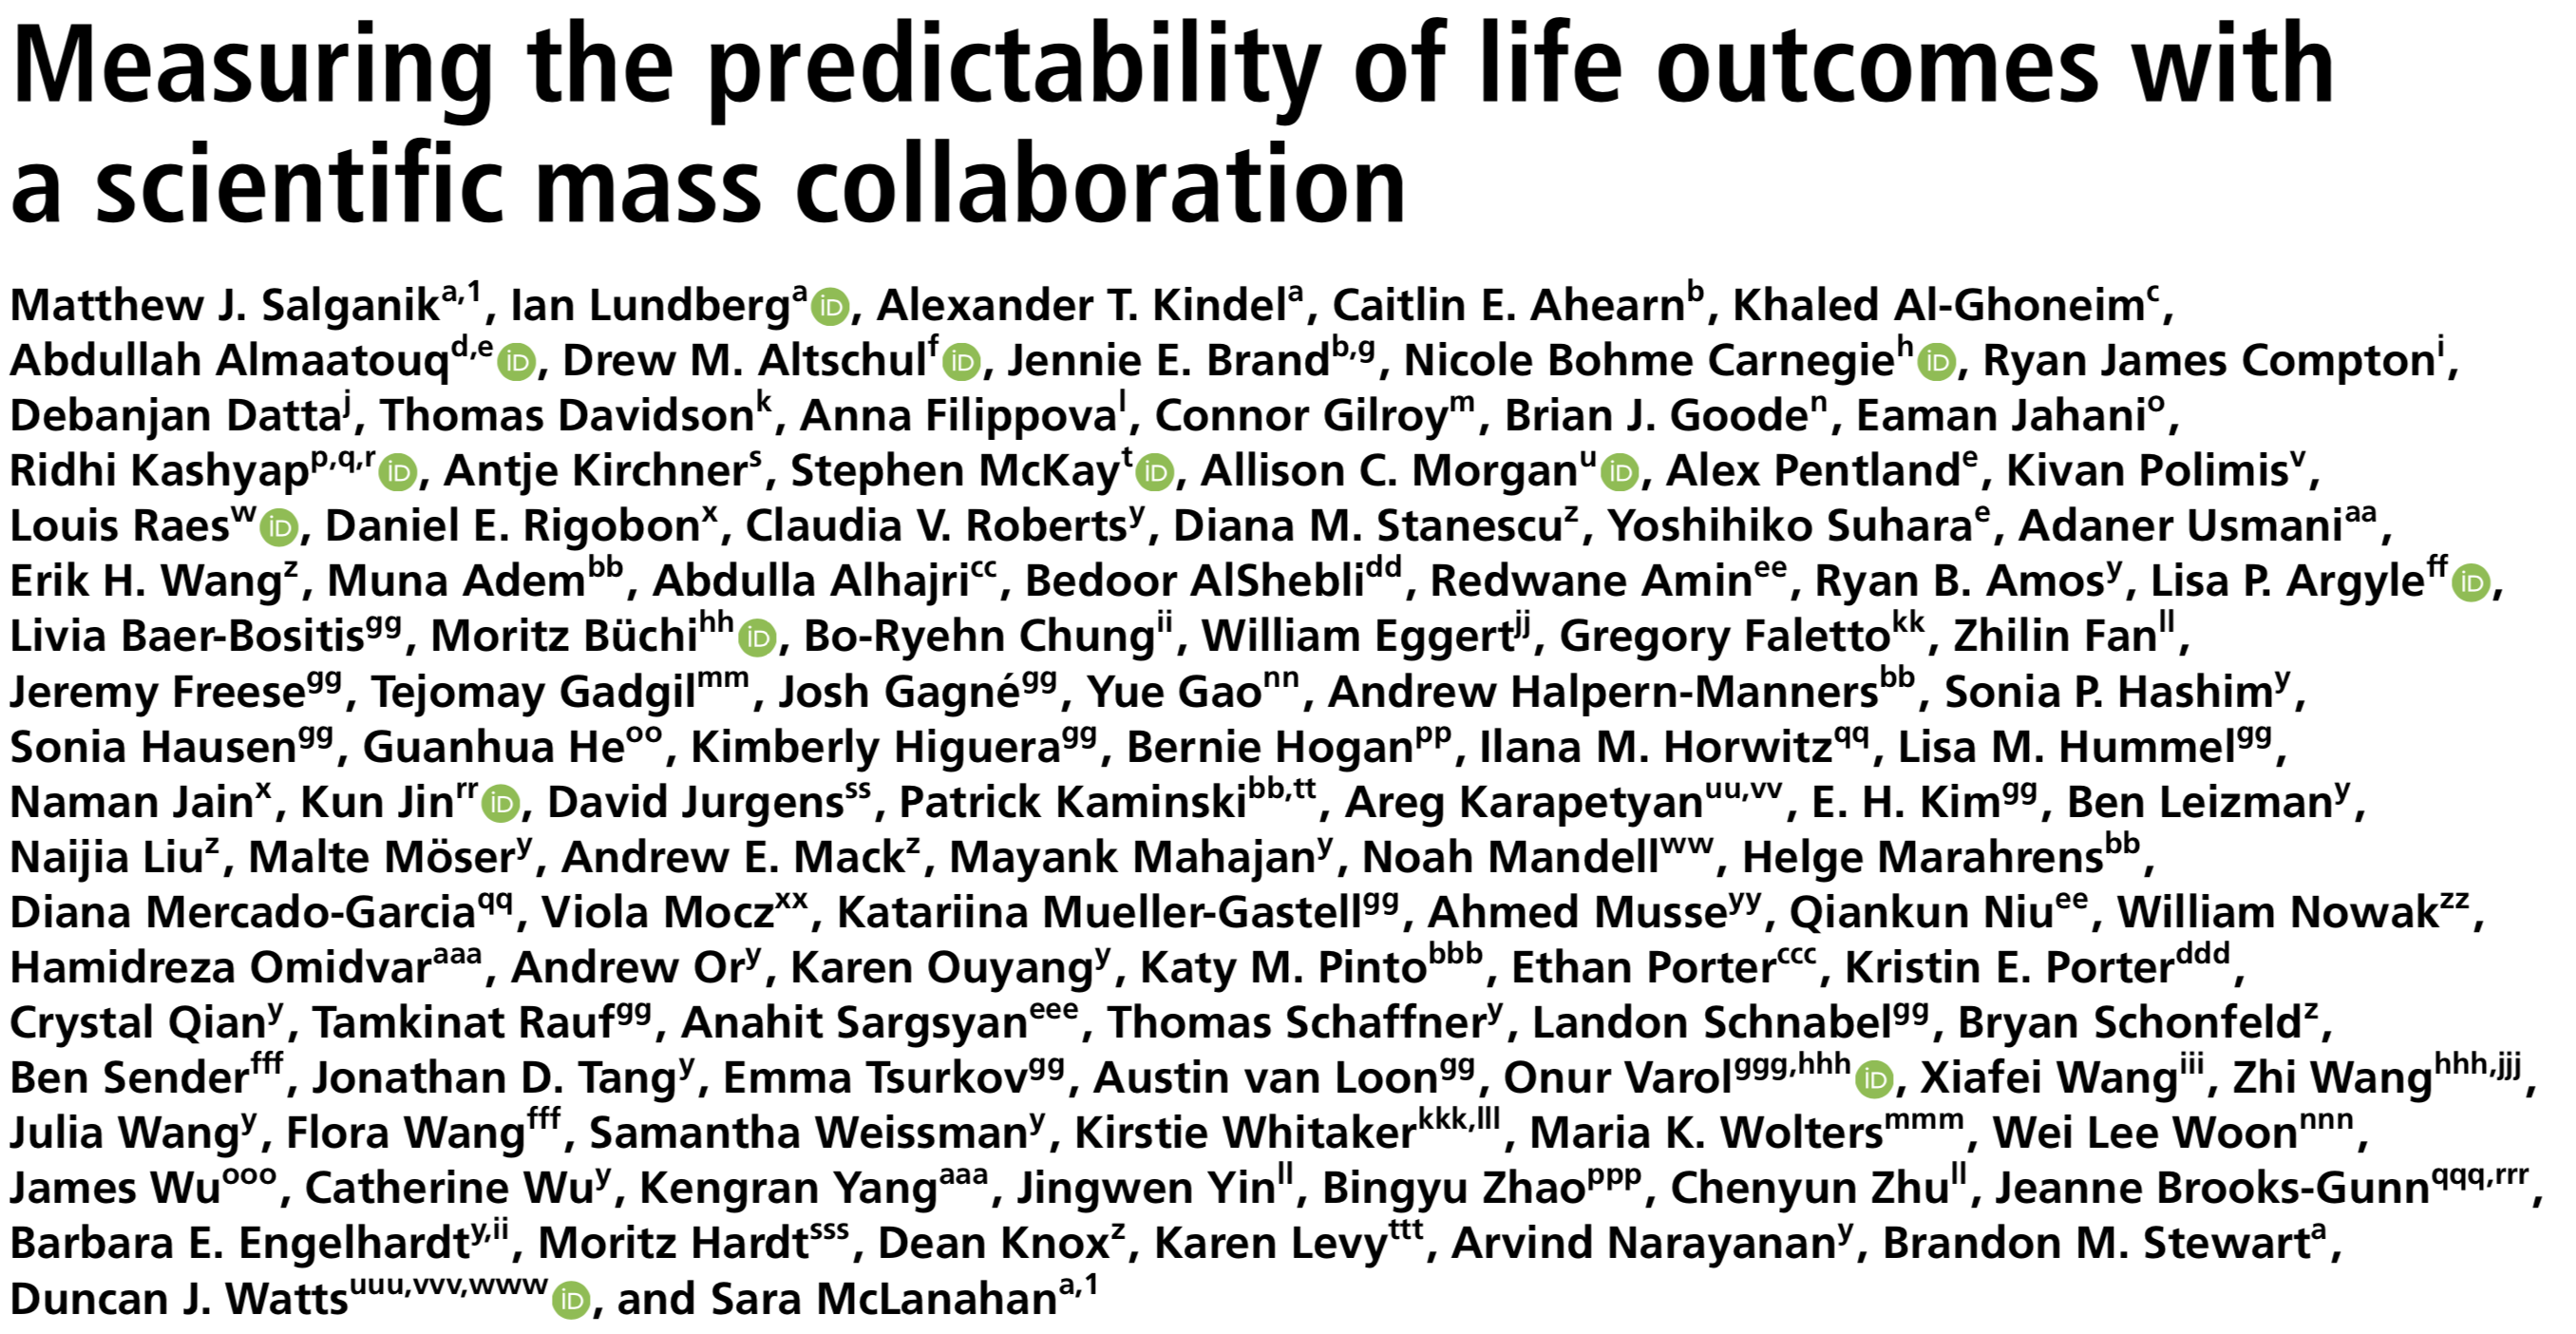
\includegraphics[width=0.9\textwidth]{figures/salganik_measuring_2020_title_authors}
\end{center}

\vfill
\url{https://doi.org/10.1073/pnas.1915006117}\\
See also Garip (2020) ``What failure to predict life outcomes can teach us'' \url{https://doi.org/10.1073/pnas.2003390117}

\end{frame}
%%%%%%%%%%%%%%%%%%%%%%%%%%%
\begin{frame}

\href{https://journals.sagepub.com/topic/collections-srd/srd-1-fragile_families/srd}{Special Collection of \textit{Socius} about the Fragile Families Challenge}
\begin{itemize}
\item 12 submitted manuscripts from Challenge participants (all with accompanying code and computing environment) \pause
\item 3 papers from our group \pause
\begin{itemize}
\item ``\href{https://doi.org/10.1177/2378023118813023}{Privacy, ethics, and data access: A case study of the Fragile Families Challenge}'' by Lundberg, Narayanan, Levy, \& Salganik \pause
\item ``\href{https://doi.org/10.1177/2378023118817378}{Improving metadata infrastructure for complex surveys: Insights from the Fragile Families Challenge}'' by Kindel, Catena, Hartshorne, Jaeger, Koffman, McLanahan, Phillips, Rouhani, Vinh, \& Salganik \pause
\item ``\href{https://doi.org/10.1177/2378023119849803}{Successes and struggles with computational reproducibility in the Fragile Families Challenge}'' by Liu \& Salganik
\end{itemize}
\end{itemize}

\end{frame}
%%%%%%%%%%%%%%%%%%%%%%%%%%%
\begin{frame}

This project creates more questions than it answers. A few next questions: \pause
\begin{itemize}
\item What is the dark matter? (Dark matter team) \pause
\item What are the implications of these findings for causal inference? (Ian Lundberg et al.) \pause
\item How predictable are the other 1,500 outcomes in the year 15 data? (Emily Cantrell, Pranay Anchuri) \pause
\item What are the implications of these findings for policy makers considering using algorithmic predictions in high-stakes decisions? (Mihir Kshirsagar et al.) \pause
\end{itemize}
\pause
A new class:
\begin{itemize}
\item COS 597E/SOC 555 Limits to Prediction (Fall 2020), Taught by Arvind Narayanan and Matthew Salganik
\end{itemize}

\end{frame}
%%%%%%%%%%%%%%%%%%%%%%%%%%%%
\begin{frame}

\begin{center}
\LARGE{
$ \hat{y} \quad \& \quad \hat{\beta}$
}
\end{center}

\vfill
\small{Mullainathan and Spiess (2017): \url{http://dx.doi.org/10.1257/jep.31.2.87}}
\end{frame}
%%%%%%%%%%%%%%%%%%%%%%%%%%
\begin{frame}

\begin{center}
\includegraphics[width=0.6\textwidth]{figures/wikipedia_logo}
\end{center}

\end{frame}
%%%%%%%%%%%%%%%%%%%%%%%%%%
\end{document}

